% Copyright 2006 by Till Tantau
%
% This file may be distributed and/or modified
%
% 1. under the LaTeX Project Public License and/or
% 2. under the GNU Free Documentation License.
%
% See the file doc/generic/pgf/licenses/LICENSE for more details.


% \section{Tutorial: A Petri-Net for Hagen}
\section{教程:哈根的Petri网}

% In this second tutorial we explore the node mechanism of \tikzname\ and \pgfname.

在第二篇教程中,我们探讨\tikzname\ 和\pgfname 节点的原理。

% Hagen must give a talk tomorrow about his favorite formalism for distributed systems: Petri nets! Hagen used to give his talks using a blackboard and everyone seemed to be perfectly content with this. Unfortunately, his audience has been spoiled recently with fancy projector-based presentations and there seems to be a certain amount of peer pressure that his Petri nets should also be drawn using a graphic program. One of the professors at his institute recommends \tikzname\ for this and Hagen decides to give it a try.

哈根(Hagen)明天需要就他最喜欢的分布式系统形式:Petri网发表演讲。 哈根以前常常用黑板发表演讲,每个人似乎对此都很满意。 不幸的是,他的听众最近迷恋上了基于投影仪的奇特演示,似乎还有一定的同行压力,要求他的Petri网的图形也应使用图形程序绘制。 为此,他所在学院的一位教授推荐了\tikzname\ ,哈根决定尝试一下。


% \subsection{Problem Statement}
\subsection{问题陈述}

% For his talk, Hagen wishes to create a graphic that demonstrates how a net with place capacities can be simulated by a net without capacities. The graphic should look like this, ideally:

对于他的演讲,哈根希望创建一个图形来演示如何通过无库所容量的网络模拟有库所容量的网络。 图形在理想情况下应该看起来像这样:{\color{red}\ref{error}}

%
\begin{quote}
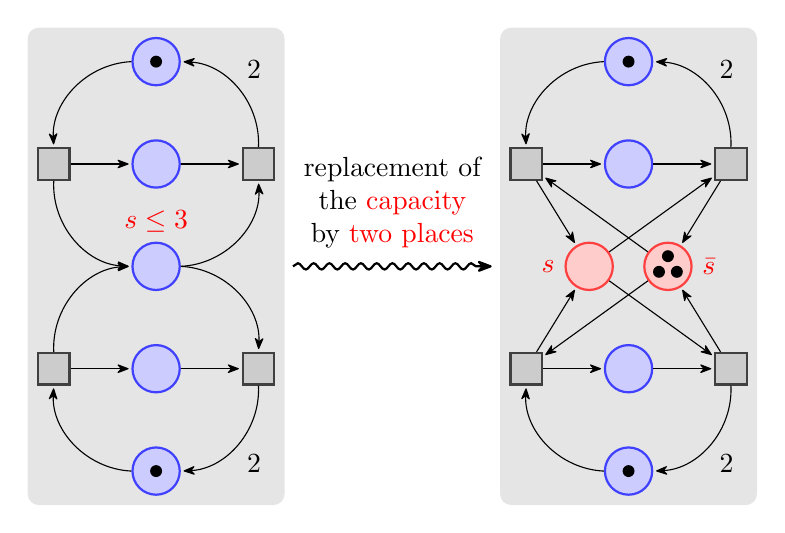
\begin{tikzpicture}
  [node distance=1.3cm,>={Stealth[round]},bend angle=45,auto,
   place/.style={circle,thick,draw=blue!75,fill=blue!20,minimum size=6mm},
   red place/.style={place,draw=red!75,fill=red!20},
   transition/.style={rectangle,thick,draw=black!75,fill=black!20,minimum size=4mm},
   every label/.style={red},on grid]

  \begin{scope}
    % First net
    \node [place,tokens=1] (w1)                                    {};
    \node [place] (c1) [below=of w1]                      {};
    \node [place] (s)  [below=of c1,label=above:$s\le 3$] {};
    \node [place] (c2) [below=of s]                       {};
    \node [place,tokens=1] (w2) [below=of c2]                      {};

    \node [transition] (e1) [left=of c1] {}
      edge [pre,bend left]                  (w1)
      edge [post,bend right]                (s)
      edge [post]                           (c1);

    \node [transition] (e2) [left=of c2] {}
      edge [pre,bend right]                 (w2)
      edge [post,bend left]                 (s)
      edge [post]                           (c2);

    \node [transition] (l1) [right=of c1] {}
      edge [pre]                            (c1)
      edge [pre,bend left]                  (s)
      edge [post,bend right] node[swap] {2} (w1);

    \node [transition] (l2) [right=of c2] {}
      edge [pre]                            (c2)
      edge [pre,bend right]                 (s)
      edge [post,bend left]  node {2}       (w2);
  \end{scope}

  \begin{scope}[xshift=6cm]
    % Second net
    \node [place,tokens=1]
                      (w1')                                                {};
    \node [place]     (c1') [below=of w1']                                 {};
    \node [red place] (s1') [below=of c1',xshift=-5mm,label=left:$s$]      {};
    \node [red place,tokens=3]
                      (s2') [below=of c1',xshift=5mm,label=right:$\bar s$] {};
    \node [place]     (c2') [below=of s1',xshift=5mm]                      {};
    \node [place,tokens=1]
                      (w2') [below=of c2']                                 {};

    \node [transition] (e1') [left=of c1'] {}
      edge [pre,bend left]                  (w1')
      edge [post]                           (s1')
      edge [pre]                            (s2')
      edge [post]                           (c1');

    \node [transition] (e2') [left=of c2'] {}
      edge [pre,bend right]                 (w2')
      edge [post]                           (s1')
      edge [pre]                            (s2')
      edge [post]                           (c2');

    \node [transition] (l1') [right=of c1'] {}
      edge [pre]                            (c1')
      edge [pre]                            (s1')
      edge [post]                           (s2')
      edge [post,bend right] node[swap] {2} (w1');

    \node [transition] (l2') [right=of c2'] {}
      edge [pre]                            (c2')
      edge [pre]                            (s1')
      edge [post]                           (s2')
      edge [post,bend left]  node {2}       (w2');
  \end{scope}

  \begin{scope}[on background layer]
    \node (r1) [fill=black!10,rounded corners,fit=(w1)(w2)(e1)(e2)(l1)(l2)] {};
    \node (r2) [fill=black!10,rounded corners,fit=(w1')(w2')(e1')(e2')(l1')(l2')] {};
  \end{scope}

  \draw [shorten >=1mm,->,thick,decorate,decoration={snake,amplitude=.4mm,segment
      length=2mm,pre=moveto,pre length=1mm,post length=2mm}]
    (r1) -- (r2)
    node [above=1mm,midway,text width=3cm,align=center]
      {replacement of the \textcolor{red}{capacity} by \textcolor{red}{two places}};

\end{tikzpicture}
\end{quote}


% \subsection{Setting up the Environment}
\subsection{配置环境}

% For the picture Hagen will need to load the \tikzname\ package as did Karl in the previous tutorial. However, Hagen will also need to load some additional \emph{library packages} that Karl did not need. These library packages contain additional definitions like extra arrow tips that are typically not needed in a picture and that need to be loaded explicitly.

为了绘制图片哈根将需要加载\tikzname\ 包,就像在以前的教程中卡尔做的那样。然而,哈根也将需要加载一些卡尔不需要的额外的\emph{库包}。这些库宏包包含额外的定义,比如图片中通常不需要的额外箭头提示,需要显式加载。

% Hagen will need to load several libraries: The |arrows.meta| library for the special arrow tip used in the graphic, the |decorations.pathmorphing| library for the ``snaking line'' in the middle, the |backgrounds| library for the two rectangular areas that are behind the two main parts of the picture, the |fit| library to easily compute the sizes of these rectangles, and the |positioning| library for placing nodes relative to other nodes.

哈根将需要加载几个库:|arrow.meta| 库用于图形中使用的特殊箭头,|decorations.pathmorphing| 库用于图形中间的``蛇形线'',|backgrounds| 库用于添加两个矩形区域后面的背景图片,|fit| 库用来轻松计算这些矩形的大小,以及 |positioning| 库将节点放置在相对于其它节点的位置上。


\subsubsection{在\LaTeX 中配置环境}

% When using \LaTeX\ use:

使用\LaTeX\ 时,请使用:

%
\begin{codeexample}[code only]
\documentclass{article} % say

\usepackage{tikz}
\usetikzlibrary{arrows.meta,decorations.pathmorphing,backgrounds,positioning,fit,petri}

\begin{document}
\begin{tikzpicture}
  \draw (0,0) -- (1,1);
\end{tikzpicture}
\end{document}
\end{codeexample}


\subsubsection{在Plain \TeX 中配置环境}

% When using Plain \TeX\ use:

使用Plain \TeX\ 时,请使用:

%
\begin{codeexample}[code only]
%% Plain TeX file
\input tikz.tex
\usetikzlibrary{arrows.meta,decorations.pathmorphing,backgrounds,positioning,fit,petri}
\baselineskip=12pt
\hsize=6.3truein
\vsize=8.7truein
\tikzpicture
  \draw (0,0) -- (1,1);
\endtikzpicture
\bye
\end{codeexample}


\subsubsection{在Con\TeX t 中配置环境}

% When using Con\TeX t, use:

使用Con\TeX t 时,请使用:

%
\begin{codeexample}[code only]
%% ConTeXt file
\usemodule[tikz]
\usetikzlibrary[arrows,decorations.pathmorphing,backgrounds,positioning,fit,petri]

\starttext
  \starttikzpicture
    \draw (0,0) -- (1,1);
  \stoptikzpicture
\stoptext
\end{codeexample}


% \subsection{Introduction to Nodes}
\subsection{节点简介}

% In principle, we already know how to create the graphics that Hagen desires (except perhaps for the snaked line, we will come to that): We start with big light gray rectangle and then add lots of circles and small rectangle, plus some arrows.

原则上,我们已经知道如何创建哈根想要的图形(也许除了蛇形线之外,我们将介绍到该图形):我们从大的浅灰色矩形开始,然后添加许多圆形和小矩形以及一些箭头。

% However, this approach has numerous disadvantages: First, it is hard to change anything at a later stage. For example, if we decide to add more places to the Petri nets (the circles are called places in Petri net theory), all of the coordinates change and we need to recalculate everything. Second, it is hard to read the code for the Petri net as it is just a long and complicated list of coordinates and drawing commands -- the underlying structure of the Petri net is lost.

但是,这种方法有许多缺点:首先,很难在以后更改任何内容。 例如,如果我们决定向Petri网添加更多的库所(在Petri网理论中圆形节点被称为库所),则所有坐标都会改变,因此我们需要重新计算所有内容。 其次,很难读取Petri网的代码,因为它只是一长串复杂的坐标和绘制命令列表——Petri网的底层结构丢失了。

% Fortunately, \tikzname\ offers a powerful mechanism for avoiding the above problems: nodes. We already came across nodes in the previous tutorial, where we used them to add labels to Karl's graphic. In the present tutorial we will see that nodes are much more powerful.

幸运的是,\tikzname\ 提供了一种避免上述问题的强大机制:节点。 在上一教程中,我们已经遇到了节点,我们使用它们在卡尔的图形中添加标签。 在本教程中,我们将看到节点功能更加强大。

% A node is a small part of a picture. When a node is created, you provide a position where the node should be drawn and a \emph{shape}. A node of shape |circle| will be drawn as a circle, a node of shape |rectangle| as a rectangle, and so on. A node may also contain some text, which is why Karl used nodes to show text. Finally, a node can get a \emph{name} for later reference.

节点只是图片的一小部分。 创建节点后,将提供一个应绘制该节点的位置和一个\emph{形状}。|circle| 形状的节点将被绘制为圆形,|rectangle| 形状的节点将被绘制为矩形等。 一个节点可能还包含一些文本,这就是卡尔可以使用节点显示文本的原因。 最后,节点还可以取一个\emph{名字}供以后参考。

% In Hagen's picture we will use nodes for the places and for the transitions of the Petri net (the places are the circles, the transitions are the rectangles). Let us start with the upper half of the left Petri net. In this upper half we have three places and two transitions. Instead of drawing three circles and two rectangles, we use three nodes of shape |circle| and two nodes of shape |rectangle|.

在哈根的图片中,我们将使用节点作为Petri网的库所和变迁(库所为圆​​形,变迁为矩形)。 让我们从左边的Petri网的上半部分开始。 在上半部分,我们有3个库所和2个变迁。我们没有画三个圆和两个矩形,而是用了三个形状为 |circ| 的节点和两个形状为 |rectangle| 的节点。

%
\begin{codeexample}[]
\begin{tikzpicture}
  \path ( 0,2) node [shape=circle,draw] {}
        ( 0,1) node [shape=circle,draw] {}
        ( 0,0) node [shape=circle,draw] {}
        ( 1,1) node [shape=rectangle,draw] {}
        (-1,1) node [shape=rectangle,draw] {};
\end{tikzpicture}
\end{codeexample}

% Hagen notes that this does not quite look like the final picture, but it seems like a good first step.

哈根指出,这看起来不太像是最终的图片,但似乎是一个不错的开始。

% Let us have a more detailed look at the code. The whole picture consists of a single path. Ignoring the |node| operations, there is not much going on in this path: It is just a sequence of coordinates with nothing ``happening'' between them. Indeed, even if something were to happen like a line-to or a curve-to, the |\path| command would not ``do'' anything with the resulting path. So, all the magic must be in the |node| commands.

让我们更详细地查看代码。整个图形由一条路径组成。忽略 |node| 操作,在这条路径上没有发生太多事情:它只是一个坐标序列,它们之间没有``发生''任何事。实际上,即使出现了像line-to或curve-to之类的命令,|\path| 命令也不会对生成的路径``做''任何事。因此,所有的魔法都存在于 |node| 命令中。

% In the previous tutorial we learned that a |node| will add a piece of text at the last coordinate. Thus, each of the five nodes is added at a different position. In the above code, this text is empty (because of the empty |{}|). So, why do we see anything at all? The answer is the |draw| option for the |node| operation: It causes the ``shape around the text'' to be drawn.

在上一个教程中,我们了解到 |node| 将在最后一个坐标处添加一段文本。 因此,五个节点中的每个节点的文本都将添加在不同的位置。 在上面的代码中,该文本为空(由于 |{}| 为空)。 那么,为什么我们什么都看不到? 答案是 |node| 操作的 |draw| 选项:它使``形状周围的文本''被绘制。

% So, the code |(0,2) node [shape=circle,draw] {}| means the following: ``In the main path, add a move-to to the coordinate |(0,2)|. Then, temporarily suspend the construction of the main path while the node is built. This node will be a |circle| around an empty text. This circle is to be |draw|n, but not filled or otherwise used. Once this whole node is constructed, it is saved until after the main path is finished. Then, it is drawn.'' The following |(0,1) node [shape=circle,draw] {}| then has the following effect: ``Continue the main path with a move-to to |(0,1)|. Then construct a node at this position also. This node is also shown after the main path is finished.'' And so on.

因此,代码 |(0,2) node [shape=circle,draw] {}| 表示: ``在主路径中,首先将笔移动到坐标为 |(0,2)| 的位置。 然后,在创建节点时临时中止主路径的创建。 该节点是绘制在一个空文本周围的 |circ| 节点。该圆将被绘出,但并没有被填充或进行其它操作。 创建整个节点后,将保存该节点,直到完成主路径为止。'' 接下来的 |(0,1) node [shape=circle,draw] {}| 类似地产生以下效果:``通过将笔移至坐标为 |(0,1)| 的位置后继续绘制主路径。 然后在此位置也构造一个节点。 主路径完成后也会显示该节点。'' 以此类推。


% \subsection{Placing Nodes Using the At Syntax}
\subsection{使用At语法放置节点}

% Hagen now understands how the |node| operation adds nodes to the path, but it seems a bit silly to create a path using the |\path| operation, consisting of numerous superfluous move-to operations, only to place nodes. He is pleased to learn that there are ways to add nodes in a more sensible manner.

哈根现在了解 |node| 操作将节点添加到路径,但是使用 |\path| 操作创建路径似乎有点愚蠢。包括许多多余的move-to操作,仅用于放置节点。 他很高兴得知有一些方法可以以更明智的方式添加节点。

% First, the |node| operation allows one to add |at (|\meta{coordinate}|)| in order to directly specify where the node should be placed, sidestepping the rule that nodes are placed on the last coordinate. Hagen can then write the following:

首先,|node| 操作允许添加 |at (|\meta{coordinate}|)|,以便直接指定节点的位置,避免节点放置在最后一个坐标上。哈根然后可以据此编写以下内容:

%
\begin{codeexample}[]
\begin{tikzpicture}
  \path node at ( 0,2) [shape=circle,draw] {}
        node at ( 0,1) [shape=circle,draw] {}
        node at ( 0,0) [shape=circle,draw] {}
        node at ( 1,1) [shape=rectangle,draw] {}
        node at (-1,1) [shape=rectangle,draw] {};
\end{tikzpicture}
\end{codeexample}

% Now Hagen is still left with a single empty path, but at least the path no longer contains strange move-to's. It turns out that this can be improved further: The |\node| command is an abbreviation for |\path node|, which allows Hagen to write:

现在,哈根仍然只剩下一条空的路径,但至少该路径不再包含奇怪的move-to路线。 事实证明,这可以进一步改进:|\node| 命令是 |\path node| 的缩写,这允许哈根这样编写:

%
\begin{codeexample}[]
\begin{tikzpicture}
  \node at ( 0,2) [circle,draw] {};
  \node at ( 0,1) [circle,draw] {};
  \node at ( 0,0) [circle,draw] {};
  \node at ( 1,1) [rectangle,draw] {};
  \node at (-1,1) [rectangle,draw] {};
\end{tikzpicture}
\end{codeexample}

% Hagen likes this syntax much better than the previous one. Note that Hagen has also omitted the |shape=| since, like |color=|, \tikzname\ allows you to omit the |shape=| if there is no confusion.

相比于之前,哈根更喜欢现在这种语法。 注意,哈根还省略了 |shape=|, 与 |color=| 一样,\tikzname\ 允许您在不引起混乱的情况下省略 |shape=|。


% \subsection{Using Styles}
\subsection{使用样式}

% Feeling adventurous, Hagen tries to make the nodes look nicer. In the final picture, the circles and rectangle should be filled with different colors, resulting in the following code:

出于冒险的感觉,哈根试图让节点看起来更好。在最终的图片中,圆和矩形需要用不同的颜色填充,从而产生以下代码:

%
\begin{codeexample}[]
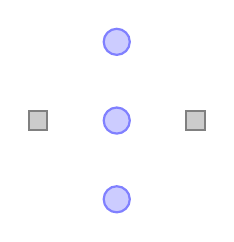
\begin{tikzpicture}[thick]
  \node at ( 0,2) [circle,draw=blue!50,fill=blue!20] {};
  \node at ( 0,1) [circle,draw=blue!50,fill=blue!20] {};
  \node at ( 0,0) [circle,draw=blue!50,fill=blue!20] {};
  \node at ( 1,1) [rectangle,draw=black!50,fill=black!20] {};
  \node at (-1,1) [rectangle,draw=black!50,fill=black!20] {};
\end{tikzpicture}
\end{codeexample}

% While this looks nicer in the picture, the code starts to get a bit ugly. Ideally, we would like our code to transport the message ``there are three places and two transitions'' and not so much which filling colors should be used.

虽然这在图片中看起来更好,但是代码开始变得有些难看。 理想情况下,我们希望代码传递``有三个库所和两个变迁''的消息,而不是要使用哪种填充颜色。

% To solve this problem, Hagen uses styles. He defines a style for places and another style for transitions:

为了解决此问题,哈根使用了样式。 他为库所定义了一种样式,为变迁定义了另一种样式:

%
\begin{codeexample}[]
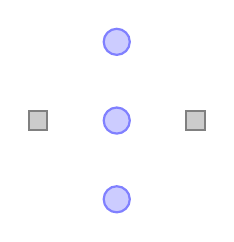
\begin{tikzpicture}
  [place/.style={circle,draw=blue!50,fill=blue!20,thick},
   transition/.style={rectangle,draw=black!50,fill=black!20,thick}]
  \node at ( 0,2) [place] {};
  \node at ( 0,1) [place] {};
  \node at ( 0,0) [place] {};
  \node at ( 1,1) [transition] {};
  \node at (-1,1) [transition] {};
\end{tikzpicture}
\end{codeexample}


% \subsection{Node Size}
\subsection{节点尺寸}

% Before Hagen starts naming and connecting the nodes, let us first make sure that the nodes get their final appearance. They are still too small. Indeed, Hagen wonders why they have any size at all, after all, the text is empty. The reason is that \tikzname\ automatically adds some space around the text. The amount is set using the option |inner sep|. So, to increase the size of the nodes, Hagen could write:

在哈根开始命名和连接节点之前,让我们首先确定节点具有最终外观。 它们还有点太小。 的确,哈根想知道为什么它们根本没有任何尺寸,毕竟文本是空的。 原因是\tikzname\ 会在文本周围自动添加一些空格。 空格的数量是使用选项 |inner sep| 设置的。 因此,为了增加节点的大小,哈根可以这样写:

%
\begin{codeexample}[]
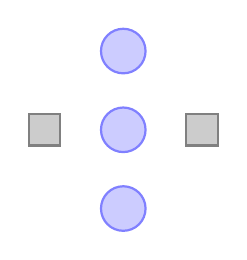
\begin{tikzpicture}
  [inner sep=2mm,
   place/.style={circle,draw=blue!50,fill=blue!20,thick},
   transition/.style={rectangle,draw=black!50,fill=black!20,thick}]
  \node at ( 0,2) [place] {};
  \node at ( 0,1) [place] {};
  \node at ( 0,0) [place] {};
  \node at ( 1,1) [transition] {};
  \node at (-1,1) [transition] {};
\end{tikzpicture}
\end{codeexample}

% However, this is not really the best way to achieve the desired effect. It is much better to use the |minimum size| option instead. This option allows Hagen to specify a minimum size that the node should have. If the node actually needs to be bigger because of a longer text, it will be larger, but if the text is empty, then the node will have |minimum size|. This option is also useful to ensure that several nodes containing different amounts of text have the same size. The options |minimum height| and |minimum width| allow you to specify the minimum height and width independently.

但是,这实际上并不是达到预期效果的最佳方法。 最好使用 |minimum size| 选项。 该选项允许哈根指定节点应具有的最小尺寸。 如果由于文本较长而实际上需要增大该节点,则该节点将变大,但是如果文本为空,则该节点将具有 |minimum size|。 这个选项对于确保包含不同长度的文本的几个节点具有相同的大小也很有用。 |minimum height| 和 |minimum width| 选项还允许您独立指定最小高度和最小宽度。

% So, what Hagen needs to do is to provide |minimum size| for the nodes. To be on the safe side, he also sets |inner sep=0pt|. This ensures that the nodes will really have size |minimum size| and not, for very small minimum sizes, the minimal size necessary to encompass the automatically added space.

因此,哈根需要做的就是给节点提供|minimum size|。 为了安全起见,他还设置了 |inner sep=0pt|。 这样可以确保节点真正具有|minimum size|。 而对于设置的非常小的的最小尺寸,节点并不是具有这个最小尺寸,而是包含自动添加的空间所需的最小尺寸。 

%
\begin{codeexample}[]
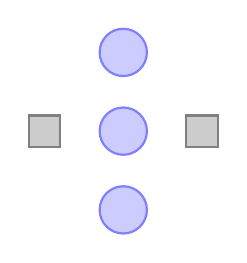
\begin{tikzpicture}
  [place/.style={circle,draw=blue!50,fill=blue!20,thick,
                 inner sep=0pt,minimum size=6mm},
   transition/.style={rectangle,draw=black!50,fill=black!20,thick,
                      inner sep=0pt,minimum size=4mm}]
  \node at ( 0,2) [place] {};
  \node at ( 0,1) [place] {};
  \node at ( 0,0) [place] {};
  \node at ( 1,1) [transition] {};
  \node at (-1,1) [transition] {};
\end{tikzpicture}
\end{codeexample}


% \subsection{Naming Nodes}
\subsection{节点命名}

% Hagen's next aim is to connect the nodes using arrows. This seems like a tricky business since the arrows should not start in the middle of the nodes, but somewhere on the border and Hagen would very much like to avoid computing these positions by hand.

哈根的下一个目标是使用箭头连接节点。 这似乎是一项棘手的工作,因为箭头不应从节点的中间开始,而是边界上的某个地方,哈根非常希望避免手动计算这些位置。

% Fortunately, \pgfname\ will perform all the necessary calculations for him. However, he first has to assign names to the nodes so that he can reference them later on. 

幸运的是,\pgfname\ 将为他执行所有必要的计算。 但是,他首先必须为节点分配名称,以便以后可以引用它们。

% There are two ways to name a node. The first is to use the |name=| option. The second method is to write the desired name in parentheses after the |node| operation. Hagen thinks that this second method seems strange, but he will soon change his opinion.

命名节点有两种方法。 第一种是使用 |name=| 选项。 第二种方法是在 |node| 操作之后的括号中写入节点的名称。哈根认为第二种方法似乎很奇怪,但是他很快就会改变看法。

%
\begin{codeexample}[setup code,hidden]
\tikzset{
    place/.style={circle,draw=blue!50,fill=blue!20,thick,
                  inner sep=0pt,minimum size=6mm},
    transition/.style={rectangle,draw=black!50,fill=black!20,thick,
                       inner sep=0pt,minimum size=4mm}
}
\end{codeexample}
%
\begin{codeexample}[]
% ... set up styles
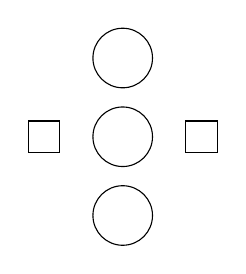
\begin{tikzpicture}
  \node (waiting 1)      at ( 0,2) [place] {};
  \node (critical 1)     at ( 0,1) [place] {};
  \node (semaphore)      at ( 0,0) [place] {};
  \node (leave critical) at ( 1,1) [transition] {};
  \node (enter critical) at (-1,1) [transition] {};
\end{tikzpicture}
\end{codeexample}

% Hagen is pleased to note that the names help in understanding the code. Names for nodes can be pretty arbitrary, but they should not contain commas, periods, parentheses, colons, and some other special characters. However, they can contain underscores and hyphens.

哈根很高兴地注意到,这些名称有助于理解代码。 节点的名称可以是任意的,但它们不应包含逗号,句点,括号,冒号和其他一些特殊字符。 但是,它们可以包含下划线和连字符。

% The syntax for the |node| operation is quite liberal with respect to the order in which node names, the |at| specifier, and the options must come. Indeed, you can even have multiple option blocks between the |node| and the text in curly braces, they accumulate. You can rearrange them arbitrarily and perhaps the following might be preferable:

|node| 操作的语法在节点名称、|at| 和必须提供的选项的顺序方面是相当自由的。实际上,你甚至可以在 |node| 和花括号文本之间有多个选项块,它们会累积。你可以随意地重新排列它们,也许下面的方法更可取:

%
\begin{codeexample}[]
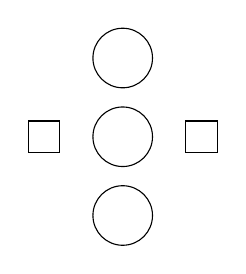
\begin{tikzpicture}
  \node[place]      (waiting 1)      at ( 0,2) {};
  \node[place]      (critical 1)     at ( 0,1) {};
  \node[place]      (semaphore)      at ( 0,0) {};
  \node[transition] (leave critical) at ( 1,1) {};
  \node[transition] (enter critical) at (-1,1) {};
\end{tikzpicture}
\end{codeexample}


% \subsection{Placing Nodes Using Relative Placement}
\subsection{使用相对位置放置节点}

% Although Hagen still wishes to connect the nodes, he first wishes to address another problem again: The placement of the nodes. Although he likes the |at| syntax, in this particular case he would prefer placing the nodes ``relative to each other''. So, Hagen would like to say that the |critical 1| node should be below the |waiting 1| node, wherever the |waiting 1| node might be. There are different ways of achieving this, but the nicest one in Hagen's case is the |below| option:

尽管哈根仍然希望连接节点,但他首先希望再次解决另一个问题:节点的放置。 尽管他喜欢 |at| 语法,在这种情况下,他宁愿将节点``彼此相对''地进行放置。 因此,哈根想说 |critical 1| 节点应在 |waiting 1| 节点的下方,无论 |waiting 1| 节点可能在哪个位置。 有多种方法可以实现此目的,但是在哈根的案例中,最好的方法是使用 |belloe| 选项:

%
\begin{codeexample}[preamble={\usetikzlibrary{positioning}}]
\begin{tikzpicture}
  \node[place]      (waiting)                            {};
  \node[place]      (critical)       [below=of waiting]  {};
  \node[place]      (semaphore)      [below=of critical] {};
  \node[transition] (leave critical) [right=of critical] {};
  \node[transition] (enter critical) [left=of critical]  {};
\end{tikzpicture}
\end{codeexample}

% With the |positioning| library loaded, when an option like |below| is followed by |of|, then the position of the node is shifted in such a manner that it is placed at the distance |node distance| in the specified direction of the given direction. The |node distance| is either the distance between the centers of the nodes (when the |on grid| option is set to true) or the distance between the borders (when the |on grid| option is set to false, which is the default).

加载 |positioning| 库后,当 |bellow| 选项后面跟着 |of| 时,则将节点的位置移动到指定方向,使其置于与指定节点的距离为 |node distance| 的位置。|node distance| 要么是节点中心之间的距离(当 |on grid| 选项被设置为true时),要么是边界之间的距离(当 |on grid| 选项被设置为false时,这是默认值)。

% Even though the above code has the same effect as the earlier code, Hagen can pass it to his colleagues who will be able to just read and understand it, perhaps without even having to see the picture.

即使上面的代码与早期的代码具有相同的效果,哈根仍可以将其传递给他的同事,他们甚至可以不必看图片就可以阅读和理解它。


% \subsection{Adding Labels Next to Nodes}
\subsection{在节点旁添加标签}

% Before we have a look at how Hagen can connect the nodes, let us add the capacity ``$s \le 3$'' to the bottom node. For this, two approaches are possible:

在查看哈根如何连接节点之前,让我们将容量``$s \le 3$''添加到底部节点。 为此,可以采用两种方法:

%
\begin{enumerate}
    % \item Hagen can just add a new node above the |north| anchor of the |semaphore| node.
    \item 哈根只需要在 |semaphore| 节点的 |north| 锚点上方添加一个新节点。
    %
\begin{codeexample}[preamble={\usetikzlibrary{positioning}}]
\begin{tikzpicture}
  \node[place]      (waiting)                            {};
  \node[place]      (critical)       [below=of waiting]  {};
  \node[place]      (semaphore)      [below=of critical] {};
  \node[transition] (leave critical) [right=of critical] {};
  \node[transition] (enter critical) [left=of critical]  {};

  \node [red,above] at (semaphore.north) {$s\le 3$};
\end{tikzpicture}
\end{codeexample}
        %
    % This is a general approach that will ``always work''.

    这是一种将``始终有效''的通用方法。

    % \item Hagen can use the special |label| option. This option is given to a |node| and it causes \emph{another} node to be added next to the node where the option is given. Here is the idea: When we construct the |semaphore| node, we wish to indicate that we want another node with the capacity above it. For this, we use the option |label=above:$s\le 3$|. This option is interpreted as follows: We want a node above the |semaphore| node and this node should read ``$s \le 3$''. Instead of |above| we could also use things like |below left| before the colon or a number like |60|.
    \item 哈根还可以使用特殊的 |label| 选项。 该选项被赋给 |node|, 使\emph{另一个}节点被添加到给出该选项的节点旁边。 这里是一个想法:当创建 |semaphore| 节点时,我们希望表明我们想要另一个位置高于它的节点。 为此,我们使用选项 |label=above:$s\le 3$|。 此选项的解释如下:我们希望在 |semaphore| 上方有一个节点,此节点应显示为``$s \le 3$''。 除了 |above| 我们还可以在冒号或在 |60| 之类的数字之前使用 |below left|。
    %
\begin{codeexample}[preamble={\usetikzlibrary{positioning}}]
\begin{tikzpicture}
  \node[place]      (waiting)                            {};
  \node[place]      (critical)       [below=of waiting]  {};
  \node[place]      (semaphore)      [below=of critical,
                                      label=above:$s\le3$] {};
  \node[transition] (leave critical) [right=of critical] {};
  \node[transition] (enter critical) [left=of critical]  {};
\end{tikzpicture}
\end{codeexample}
        %
    % It is also possible to give multiple |label| options, this causes multiple labels to be drawn.

    也可以给多个 |label| 选项,将会绘制多个标签。
    %
\begin{codeexample}[]
\tikz
  \node [circle,draw,label=60:$60^\circ$,label=below:$-90^\circ$] {my circle};
\end{codeexample}
        %
    % Hagen is not fully satisfied with the |label| option since the label is not red. To achieve this, he has two options: First, he can redefine the |every label| style. Second, he can add options to the label's node. These options are given following the |label=|, so he would write |label=[red]above:$s\le3$|. However, this does not quite work since \TeX\ thinks that the |]| closes the whole option list of the |semaphore| node. So, Hagen has to add braces and writes |label={[red]above:$s\le3$}|. Since this looks a bit ugly, Hagen decides to redefine the |every label| style.

    哈根对 |label| 选项并不完全满意,因为标签不是红色的。为了实现这一点,他有两个选择:首先,他可以重新定义 |every label| 的风格。其次,他可以向标签的节点中添加选项。这些选项是按照 |label=| 给出的,所以他在上面写 |label=[red]above:$s\le3$|。然而,这并不能完全工作,因为\TeX\ 认为 |]| 结束了 |semaphore| 节点的整个选项列表。因此,哈根必须添加括号这样使用 |label={[red]above:$s\le3$}|。由于这看起来有点丑,哈根决定重新定义 |every label| 风格。
        %
\begin{codeexample}[preamble={\usetikzlibrary{positioning}}]
\begin{tikzpicture}[every label/.style={red}]
  \node[place]      (waiting)                            {};
  \node[place]      (critical)       [below=of waiting]  {};
  \node[place]      (semaphore)      [below=of critical,
                                      label=above:$s\le3$] {};
  \node[transition] (leave critical) [right=of critical] {};
  \node[transition] (enter critical) [left=of critical]  {};
\end{tikzpicture}
\end{codeexample}
\end{enumerate}


% \subsection{Connecting Nodes}
\subsection{连接节点}

% It is now high time to connect the nodes. Let us start with something simple, namely with the straight line from |enter critical| to |critical|. We want this line to start at the right side of |enter critical| and to end at the left side of |critical|. For this, we can use the \emph{anchors} of the nodes. Every node defines a whole bunch of anchors that lie on its border or inside it. For example, the |center| anchor is at the center of the node, the |west| anchor is on the left of the node, and so on. To access the coordinate of a node, we use a coordinate that contains the node's name followed by a dot, followed by the anchor's name:

现在是连接节点的时候了。 让我们先从简单的事情开始,即从直线的 |enter critical| 到 |critical|。 我们希望此直线从 |enter critical| 的右侧开始,并在 | critical| 的左侧结束。 为此,我们可以使用节点的\emph{锚点}。 每个节点都定义了一大堆锚点,这些锚点位于其边界上或内部。 例如,|center| 锚点位于节点的中心,|west| 锚点位于节点的左侧,依此类推。 要访问节点的坐标,我们使用一个坐标,该坐标包含节点名称,后跟一句点,再后跟锚点名称:

%
\begin{codeexample}[preamble={\usetikzlibrary{positioning}}]
\begin{tikzpicture}
  \node[place]      (waiting)                            {};
  \node[place]      (critical)       [below=of waiting]  {};
  \node[place]      (semaphore)      [below=of critical] {};
  \node[transition] (leave critical) [right=of critical] {};
  \node[transition] (enter critical) [left=of critical]  {};
  \draw [->] (critical.west) -- (enter critical.east);
\end{tikzpicture}
\end{codeexample}

% Next, let us tackle the curve from |waiting| to |enter critical|. This can be specified using curves and controls:

接下来,让我们处理从 |waiting| 到 |enter critical| 的曲线。可以使用曲线和控件来指定:

%
\begin{codeexample}[preamble={\usetikzlibrary{positioning}}]
\begin{tikzpicture}
  \node[place]      (waiting)                            {};
  \node[place]      (critical)       [below=of waiting]  {};
  \node[place]      (semaphore)      [below=of critical] {};
  \node[transition] (leave critical) [right=of critical] {};
  \node[transition] (enter critical) [left=of critical]  {};
  \draw [->] (enter critical.east) -- (critical.west);
  \draw [->] (waiting.west) .. controls +(left:5mm) and +(up:5mm)
                            .. (enter critical.north);
\end{tikzpicture}
\end{codeexample}

% Hagen sees how he can now add all his edges, but the whole process seems a but awkward and not very flexible. Again, the code seems to obscure the structure of the graphic rather than showing it.

哈根看到了他现在如何添加他所有的边,但是整个过程看起来很笨拙,不是很灵活。再次,代码似乎使图形的结构变得晦涩,而不是展示图形是如何绘制而来的。

% So, let us start improving the code for the edges. First, Hagen can leave out the anchors:

因此,让我们开始改进边的代码。 首先,哈根可以省略锚点:

%
\begin{codeexample}[preamble={\usetikzlibrary{positioning}}]
\begin{tikzpicture}
  \node[place]      (waiting)                            {};
  \node[place]      (critical)       [below=of waiting]  {};
  \node[place]      (semaphore)      [below=of critical] {};
  \node[transition] (leave critical) [right=of critical] {};
  \node[transition] (enter critical) [left=of critical]  {};
  \draw [->] (enter critical) -- (critical);
  \draw [->] (waiting) .. controls +(left:8mm) and +(up:8mm)
                       .. (enter critical);
\end{tikzpicture}
\end{codeexample}

% Hagen is a bit surprised that this works. After all, how did \tikzname\ know that the line from |enter critical| to |critical| should actually start on the borders? Whenever \tikzname\ encounters a whole node name as a ``coordinate'', it tries to ``be smart'' about the anchor that it should choose for this node. Depending on what happens next, \tikzname\ will choose an anchor that lies on the border of the node on a line to the next coordinate or control point. The exact rules are a bit complex, but the chosen point will usually be correct -- and when it is not, Hagen can still specify the desired anchor by hand.

哈根有点惊讶,这是可行的。毕竟,\tikzname\ 怎么知道从 |enter critical| 到 |critical| 的直线实际上应该从边界开始呢?每当\tikzname\ 遇到作为``坐标''的整个节点名时,它就会尝试``“''聪明地''”''为该节点选择锚点。根据接下来发生的情况,\tikzname\ 将选择位于节点边界上的锚点,该锚点位于到下一个坐标或控制点的直线上。确切的规则有点复杂,但选择的点通常是正确的,如果不是这样,哈根仍然可以手工指定所需的锚点。

% Hagen would now like to simplify the curve operation somehow. It turns out that this can be accomplished using a special path operation: the |to| operation. This operation takes many options (you can even define new ones yourself). One pair of options is useful for Hagen: The pair |in| and |out|. These options take angles at which a curve should leave or reach the start or target coordinates. Without these options, a straight line is drawn:

哈根现在想以某种方式简化曲线操作。 事实证明,这可以使用特殊的路径操作来实现:|to| 操作。 此操作有很多选项(您甚至可以自己定义新选项)。 这组选项对哈根很有用:|in| 和 |out| 组。 这些选项采用曲线应离开或到达起始坐标或目标坐标的角度。如果没有这些选项,则会绘制一条直线:

%
\begin{codeexample}[preamble={\usetikzlibrary{positioning}}]
\begin{tikzpicture}
  \node[place]      (waiting)                            {};
  \node[place]      (critical)       [below=of waiting]  {};
  \node[place]      (semaphore)      [below=of critical] {};
  \node[transition] (leave critical) [right=of critical] {};
  \node[transition] (enter critical) [left=of critical]  {};
  \draw [->] (enter critical) to                 (critical);
  \draw [->] (waiting)        to [out=180,in=90] (enter critical);
\end{tikzpicture}
\end{codeexample}

% There is another option for the |to| operation, that is even better suited to Hagen's problem: The |bend right| option. This option also takes an angle, but this angle only specifies the angle by which the curve is bent to the right:

|to| 操作还有另一种选项,它甚至更适合于哈根的问题:|bend right| 选项。 此选项也需要一个角度,但是此角度仅指定曲线向右弯曲的角度:

%
\begin{codeexample}[preamble={\usetikzlibrary{positioning}}]
\begin{tikzpicture}
  \node[place]      (waiting)                            {};
  \node[place]      (critical)       [below=of waiting]  {};
  \node[place]      (semaphore)      [below=of critical] {};
  \node[transition] (leave critical) [right=of critical] {};
  \node[transition] (enter critical) [left=of critical]  {};
  \draw [->] (enter critical) to                 (critical);
  \draw [->] (waiting)        to [bend right=45] (enter critical);
  \draw [->] (enter critical) to [bend right=45] (semaphore);
\end{tikzpicture}
\end{codeexample}

% It is now time for Hagen to learn about yet another way of specifying edges: Using the |edge| path operation. This operation is very similar to the |to| operation, but there is one important difference: Like a node the edge generated by the |edge| operation is not part of the main path, but is added only later. This may not seem very important, but it has some nice consequences. For example, every edge can have its own arrow tips and its own color and so on and, still, all the edges can be given on the same path. This allows Hagen to write the following:

现在是时候让哈根学习指定边的另一种方法了:使用 |edge| 路径操作。 此操作与 |to| 非常相似。 操作,但是有一个重要的区别:与节点一样,|edge| 操作生成的边不是主路径的一部分,而是仅在以后添加。 这看似不太重要,但是会带来一些不错的效果。 例如,每条边可以有自己的箭头提示和颜色,依此类推,而且所有边都可以在同一路径上给出。 这使哈根可以编写以下内容:

%
\begin{codeexample}[preamble={\usetikzlibrary{positioning}}]
\begin{tikzpicture}
  \node[place]      (waiting)                            {};
  \node[place]      (critical)       [below=of waiting]  {};
  \node[place]      (semaphore)      [below=of critical] {};
  \node[transition] (leave critical) [right=of critical] {};
  \node[transition] (enter critical) [left=of critical]  {}
    edge [->]               (critical)
    edge [<-,bend left=45]  (waiting)
    edge [->,bend right=45] (semaphore);
\end{tikzpicture}
\end{codeexample}

% Each |edge| caused a new path to be constructed, consisting of a |to| between the node |enter critical| and the node following the |edge| command.

每个 |edge| 都会绘制一条新路径,每条路径的命令都由 |enter critical| 节点和 |edge| 命令之后的节点组成,节点之间采用 |to| 连接。

% The finishing touch is to introduce two styles |pre| and |post| and to use the |bend angle=45| option to set the bend angle once and for all:

最后要介绍的是 |pre| 和 |post| 两种样式,并使用|bend angle=45| 选项一劳永逸地设置弯曲角度:

%
\begin{codeexample}[preamble={\usetikzlibrary{arrows.meta,positioning}}]
% Styles place and transition as before
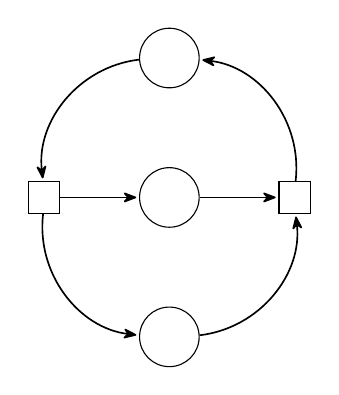
\begin{tikzpicture}
  [bend angle=45,
   pre/.style={<-,shorten <=1pt,>={Stealth[round]},semithick},
   post/.style={->,shorten >=1pt,>={Stealth[round]},semithick}]

  \node[place]      (waiting)                            {};
  \node[place]      (critical)       [below=of waiting]  {};
  \node[place]      (semaphore)      [below=of critical] {};

  \node[transition] (leave critical) [right=of critical] {}
    edge [pre]             (critical)
    edge [post,bend right] (waiting)
    edge [pre, bend left]  (semaphore);
  \node[transition] (enter critical) [left=of critical]  {}
    edge [post]            (critical)
    edge [pre, bend left]  (waiting)
    edge [post,bend right] (semaphore);
\end{tikzpicture}
\end{codeexample}


% \subsection{Adding Labels Next to Lines}
\subsection{在线旁添加标签}

% The next thing that Hagen needs to add is the ``$2$'' at the arcs. For this Hagen can use \tikzname's automatic node placement: By adding the option |auto|, \tikzname\ will position nodes on curves and lines in such a way that they are not on the curve but next to it. Adding |swap| will mirror the label with respect to the line. Here is a general example:

哈根接下来需要添加的是弧线上的``$2$''。 为此,哈根可以使用\tikzname 的自动节点放置:通过添加选项 |auto|,\tikzname\ 可以将节点定位在曲线和线上,使得它们不在曲线上而是位于曲线旁边。 添加 |swap| 将对该线的标签进行镜像。 这是一个一般示例:

%
% TODOsp: codeexamples: styles not needed here
\begin{codeexample}[]
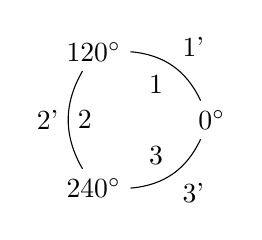
\begin{tikzpicture}[auto,bend right]
  \node (a) at (0:1) {$0^\circ$};
  \node (b) at (120:1) {$120^\circ$};
  \node (c) at (240:1) {$240^\circ$};

  \draw (a) to node {1} node [swap] {1'} (b)
        (b) to node {2} node [swap] {2'} (c)
        (c) to node {3} node [swap] {3'} (a);
\end{tikzpicture}
\end{codeexample}

% What is happening here? The nodes are given somehow inside the |to| operation! When this is done, the node is placed on the middle of the curve or line created by the |to| operation. The |auto| option then causes the node to be moved in such a way that it does not lie on the curve, but next to it. In the example we provide even two nodes on each |to| operation.  For Hagen that |auto| option is not really necessary since the two ``2'' labels could also easily be placed ``by hand''. However, in a complicated plot with numerous edges automatic placement can be a blessing.

这里发生了什么?节点以某种方式在 |to| 操作中给定!完成此操作后,节点被放置在 |to| 操作创建的曲线或直线的中间。然后,|auto| 选项导致节点以这样一种方式进行移动,即它不在曲线上,而是在曲线旁边。在本例中,我们为每个 |to| 操作提供两个节点。对于哈根来说,|auto| 选项并不是真正必要的,因为两个``2''标签也可以很容易地``手动''放置。然而,在一个有许多边的复杂情形中,自动放置可能是一件好事。

%
\begin{codeexample}[
    preamble={\usetikzlibrary{arrows.meta,positioning}},
    pre={\tikzset{
    pre/.style={<-,shorten <=1pt,>={Stealth[round]},semithick},
    post/.style={->,shorten >=1pt,>={Stealth[round]},semithick},
}},
]
% Styles as before
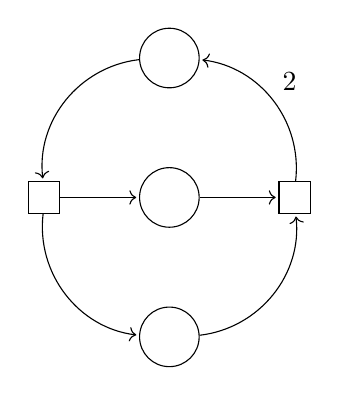
\begin{tikzpicture}[bend angle=45]
  \node[place]      (waiting)                            {};
  \node[place]      (critical)       [below=of waiting]  {};
  \node[place]      (semaphore)      [below=of critical] {};

  \node[transition] (leave critical) [right=of critical] {}
    edge [pre]                                 (critical)
    edge [post,bend right] node[auto,swap] {2} (waiting)
    edge [pre, bend left]                      (semaphore);
  \node[transition] (enter critical) [left=of critical]  {}
    edge [post]                                (critical)
    edge [pre, bend left]                      (waiting)
    edge [post,bend right]                     (semaphore);
\end{tikzpicture}
\end{codeexample}
% TODOsp: codeexamples: styles and `positioning` are needed up to here


% \subsection{Adding the Snaked Line and Multi-Line Text}
\subsection{添加隐藏线和多行文本}

% With the node mechanism Hagen can now easily create the two Petri nets. What he is unsure of is how he can create the snaked line between the nets.

利用节点机制,哈根现在可以轻松创建两个Petri网络。 他不确定的是如何在网之间创建蛇形线。

% For this he can use a \emph{decoration}. To draw the snaked line, Hagen only needs to set the two options |decoration=snake| and |decorate| on the path. This causes all lines of the path to be replaced by snakes. It is also possible to use snakes only in certain parts of a path, but Hagen will not need this. 

为此,他可以使用\emph{decoration}库。 要绘制蛇形线,哈根只需要为路径设置两个选项 |decoration=snake| 和 |decorate|。 这将导致路径的所有线都被蛇形替换。 也可以仅在路径的某些部分使用蛇形,但是哈根不需要。

\begin{codeexample}[preamble={\usetikzlibrary{decorations.pathmorphing}}]
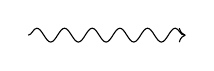
\begin{tikzpicture}
  \draw [->,decorate,decoration=snake] (0,0) -- (2,0);
\end{tikzpicture}
\end{codeexample}

% Well, that does not look quite right, yet. The problem is that the snake happens to end exactly at the position where the arrow begins. Fortunately, there is an option that helps here. Also, the snake should be a bit smaller, which can be influenced by even more options.

好吧,这看起来还不太正确。 问题是蛇形恰好在箭头开始的位置结束。 幸运的是,这里有一个选项可以帮助您。 同样,蛇形应该更小一些,这可能会受到更多选择的影响。

%
\begin{codeexample}[preamble={\usetikzlibrary{decorations.pathmorphing}}]
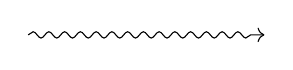
\begin{tikzpicture}
  \draw [->,decorate,
     decoration={snake,amplitude=.4mm,segment length=2mm,post length=1mm}]
    (0,0) -- (3,0);
\end{tikzpicture}
\end{codeexample}

% Now Hagen needs to add the text above the snake. This text is a bit challenging since it is a multi-line text. Hagen has two options for this: First, he can specify an |align=center| and then use the |\\| command to enforce the line breaks at the desired positions.

现在,哈根需要在蛇形上方添加文本。 该文本是多行文本,因此具有一定的挑战性。 哈根对此有两种选择:首先,他可以指定 |align=center|。 然后使用 |\\| 命令以在所需位置强制换行。

%
\begin{codeexample}[preamble={\usetikzlibrary{decorations.pathmorphing}}]
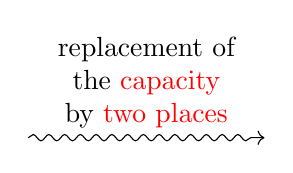
\begin{tikzpicture}
  \draw [->,decorate,
      decoration={snake,amplitude=.4mm,segment length=2mm,post length=1mm}]
    (0,0) -- (3,0)
    node [above,align=center,midway]
    {
      replacement of\\
      the \textcolor{red}{capacity}\\
      by \textcolor{red}{two places}
    };
\end{tikzpicture}
\end{codeexample}

% Instead of specifying the line breaks ``by hand'', Hagen can also specify a width for the text and let \TeX\ perform the line breaking for him:

哈根除了可以手动指定换行符之外,还可以为文本指定宽度并让\TeX\ 为他自动换行:

%
\begin{codeexample}[preamble={\usetikzlibrary{decorations.pathmorphing}}]
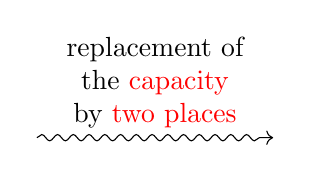
\begin{tikzpicture}
  \draw [->,decorate,
      decoration={snake,amplitude=.4mm,segment length=2mm,post length=1mm}]
    (0,0) -- (3,0)
    node [above,text width=3cm,align=center,midway]
    {
      replacement of the \textcolor{red}{capacity} by
      \textcolor{red}{two places}
    };
\end{tikzpicture}
\end{codeexample}


% \subsection{Using Layers: The Background Rectangles}
\subsection{使用图层:背景矩形}

% Hagen still needs to add the background rectangles. These are a bit tricky: Hagen would like to draw the rectangles \emph{after} the Petri nets are finished. The reason is that only then can he conveniently refer to the coordinates that make up the corners of the rectangle. If Hagen draws the rectangle first, then he needs to know the exact size of the Petri net -- which he does not.

哈根仍然需要添加背景矩形。 这些有点棘手:哈根希望在Petri网绘制完成\emph{之后}再绘制矩形。 原因是只有这样,他才能方便地得到矩形角点的坐标。如果哈根首先画出这个矩形,那么他需要知道Petri网的确切大小,但他并不知道。

% The solution is to use \emph{layers}. When the |backgrounds| library is loaded, Hagen can put parts of his picture inside a scope with the |on background layer| option. Then this part of the picture becomes part of the layer that is given as an argument to this environment. When the |{tikzpicture}| environment ends, the layers are put on top of each other, starting with the background layer. This causes everything drawn on the background layer to be behind the main text.

解决方案是使用\emph{图层}。|backgrounds| 库已加载,哈根可以将其图片的一部分放置在具有``背景层''的范围内。 然后,图片的该部分成为该环境的参数所指定的图层的一部分。 当 |{tikzpicture}| 在环境结束时,各层从背景层开始相互重叠。 这导致在背景层上绘制的所有内容都位于主文本的后面。

% The next tricky question is, how big should the rectangle be? Naturally, Hagen can compute the size ``by hand'' or using some clever observations concerning the $x$- and $y$-coordinates of the nodes, but it would be nicer to just have \tikzname\ compute a rectangle into which all the nodes ``fit''. For this, the |fit| library can be used. It defines the |fit| options, which, when given to a node, causes the node to be resized and shifted such that it exactly covers all the nodes and coordinates given as parameters to the |fit| option.

下一个棘手的问题是,矩形应该有多大? 当然,哈根可以``手工''计算大小,也可以使用一些聪明的方法来计算节点的$x$和$y$的坐标,但如果使用\tikzname\ 计算一个所有节点都适合的矩形会更好。 为此,可以使用 |fit| 库。它定义了 |fit| 选项,当将该选项提供给节点时,将对该节点的大小进行调整和移动,以便准确地覆盖作为 |fit| 选项参数提供的所有节点和坐标。

%
% TODOsp: codeexamples: redo/add styles starting from here
\begin{codeexample}[
    preamble={\usetikzlibrary{arrows.meta,backgrounds,fit,positioning}},
    pre={\tikzset{
    pre/.style={<-,shorten <=1pt,>={Stealth[round]},semithick},
    post/.style={->,shorten >=1pt,>={Stealth[round]},semithick},
}},
]
% Styles as before
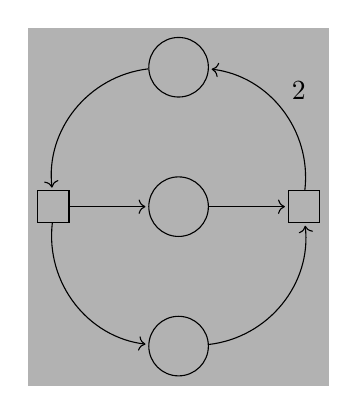
\begin{tikzpicture}[bend angle=45]
  \node[place]      (waiting)                            {};
  \node[place]      (critical)       [below=of waiting]  {};
  \node[place]      (semaphore)      [below=of critical] {};

  \node[transition] (leave critical) [right=of critical] {}
    edge [pre]                                 (critical)
    edge [post,bend right] node[auto,swap] {2} (waiting)
    edge [pre, bend left]                      (semaphore);
  \node[transition] (enter critical) [left=of critical]  {}
    edge [post]                                (critical)
    edge [pre, bend left]                      (waiting)
    edge [post,bend right]                     (semaphore);

  \begin{scope}[on background layer]
    \node [fill=black!30,fit=(waiting) (critical) (semaphore)
             (leave critical) (enter critical)] {};
  \end{scope}
\end{tikzpicture}
\end{codeexample}


% \subsection{The Complete Code}
\subsection{完整的代码}

% Hagen has now finally put everything together. Only then does he learn that there is already a library for drawing Petri nets! It turns out that this library mainly provides the same definitions as Hagen did. For example, it defines a |place| style in a similar way as Hagen did. Adjusting the code so that it uses the library shortens Hagen code a bit, as shown in the following.

哈根现在终于把所有东西都放在一起了。 这时,他才知道已经有了一个绘制Petri网的库! 事实证明,该库主要提供与哈根相同的定义。 例如,它定义了 |place|,与哈根类似。 调整代码以便使用该库,缩短了哈根的代码,如下所示。

%First, Hagen needs less style definitions, but he still needs to specify the colors of places and transitions.

首先,哈根需要较少的样式定义,但他仍然需要指定库所和变迁的颜色。

%
\begin{codeexample}[code only]
\begin{tikzpicture}
  [node distance=1.3cm,on grid,>={Stealth[round]},bend angle=45,auto,
   every place/.style=     {minimum size=6mm,thick,draw=blue!75,fill=blue!20},
   every transition/.style={thick,draw=black!75,fill=black!20},
   red place/.style=       {place,draw=red!75,fill=red!20},
   every label/.style=     {red}]
\end{codeexample}

% Now comes the code for the nets:

现在我们得到了网络的代码:

%
\ifpgfmanualexternalize\tikzexternaldisable\fi
\begin{codeexample}[
    preamble={\usetikzlibrary{arrows.meta,petri,positioning}},
    pre={\tikzset{
    every place/.style={minimum size=6mm,thick,draw=blue!75,fill=blue!20},
    every transition/.style={thick,draw=black!75,fill=black!20},
    every label/.style={red},
    every picture/.style={on grid,node distance=1.3cm,>={Stealth[round]},bend angle=45,auto},
}%
\begin{tikzpicture}},
    post={\end{tikzpicture}},
]
   \node [place,tokens=1] (w1)                                    {};
   \node [place]          (c1) [below=of w1]                      {};
   \node [place]          (s)  [below=of c1,label=above:$s\le 3$] {};
   \node [place]          (c2) [below=of s]                       {};
   \node [place,tokens=1] (w2) [below=of c2]                      {};

   \node [transition] (e1) [left=of c1] {}
     edge [pre,bend left]                  (w1)
     edge [post,bend right]                (s)
     edge [post]                           (c1);
   \node [transition] (e2) [left=of c2] {}
     edge [pre,bend right]                 (w2)
     edge [post,bend left]                 (s)
     edge [post]                           (c2);
   \node [transition] (l1) [right=of c1] {}
     edge [pre]                            (c1)
     edge [pre,bend left]                  (s)
     edge [post,bend right] node[swap] {2} (w1);
   \node [transition] (l2) [right=of c2] {}
     edge [pre]                            (c2)
     edge [pre,bend right]                 (s)
     edge [post,bend left]  node {2}       (w2);
\end{codeexample}

\ifpgfmanualexternalize\tikzexternaldisable\fi
\begin{codeexample}[
    preamble={\usetikzlibrary{arrows.meta,petri,positioning}},
    pre={\tikzset{
    every place/.style={minimum size=6mm,thick,draw=blue!75,fill=blue!20},
    every transition/.style={thick,draw=black!75,fill=black!20},
    red place/.style=  {place,draw=red!75,fill=red!20},
    every label/.style={red},
    every picture/.style={on grid,node distance=1.3cm,>={Stealth[round]},bend angle=45,auto},
}%
\begin{tikzpicture}},
    post={\end{tikzpicture}},
]
  \begin{scope}[xshift=6cm]
    \node [place,tokens=1]     (w1')                            {};
    \node [place]              (c1') [below=of w1']             {};
    \node [red place]          (s1') [below=of c1',xshift=-5mm]
            [label=left:$s$]                                    {};
    \node [red place,tokens=3] (s2') [below=of c1',xshift=5mm]
            [label=right:$\bar s$]                              {};
    \node [place]              (c2') [below=of s1',xshift=5mm]  {};
    \node [place,tokens=1]     (w2') [below=of c2']             {};

    \node [transition] (e1') [left=of c1'] {}
      edge [pre,bend left]                  (w1')
      edge [post]                           (s1')
      edge [pre]                            (s2')
      edge [post]                           (c1');
    \node [transition] (e2') [left=of c2'] {}
      edge [pre,bend right]                 (w2')
      edge [post]                           (s1')
      edge [pre]                            (s2')
      edge [post]                           (c2');
    \node [transition] (l1') [right=of c1'] {}
      edge [pre]                            (c1')
      edge [pre]                            (s1')
      edge [post]                           (s2')
      edge [post,bend right] node[swap] {2} (w1');
    \node [transition] (l2') [right=of c2'] {}
      edge [pre]                            (c2')
      edge [pre]                            (s1')
      edge [post]                           (s2')
      edge [post,bend left]  node {2}       (w2');
  \end{scope}
\end{codeexample}

% The code for the background and the snake is the following:

背景和蛇形的代码如下:

%
\begin{codeexample}[code only]
  \begin{scope}[on background layer]
    \node (r1) [fill=black!10,rounded corners,fit=(w1)(w2)(e1)(e2)(l1)(l2)] {};
    \node (r2) [fill=black!10,rounded corners,fit=(w1')(w2')(e1')(e2')(l1')(l2')] {};
  \end{scope}

  \draw [shorten >=1mm,->,thick,decorate,
         decoration={snake,amplitude=.4mm,segment length=2mm,
                     pre=moveto,pre length=1mm,post length=2mm}]
    (r1) -- (r2) node [above=1mm,midway,text width=3cm,align=center]
      {replacement of the \textcolor{red}{capacity} by \textcolor{red}{two places}};
\end{tikzpicture}
\end{codeexample}

% -----------------------------------------------------------------------------
% TODOsp: codeexamples: This is needed because -- unlike I thought --
%         `setup code is remembered also outside this file. Thus the changed
%         style of `place` and `transition` are "remembered" in
%         <pgfmanual-en-library-petri.tex>
\begin{codeexample}[setup code,hidden]
% from <tikzlibrarypetri.code.tex>
\tikzset{
    place/.style={circle,draw,inner sep=0pt,minimum size=5ex,every place},
    transition/.style={rectangle,draw,inner sep=0pt,minimum size=4mm,every transition},
}
\end{codeexample}
% -----------------------------------------------------------------------------

\clearpage